\documentclass{standalone}
\usepackage{tikz}
\usetikzlibrary{patterns, positioning}

\begin{document}
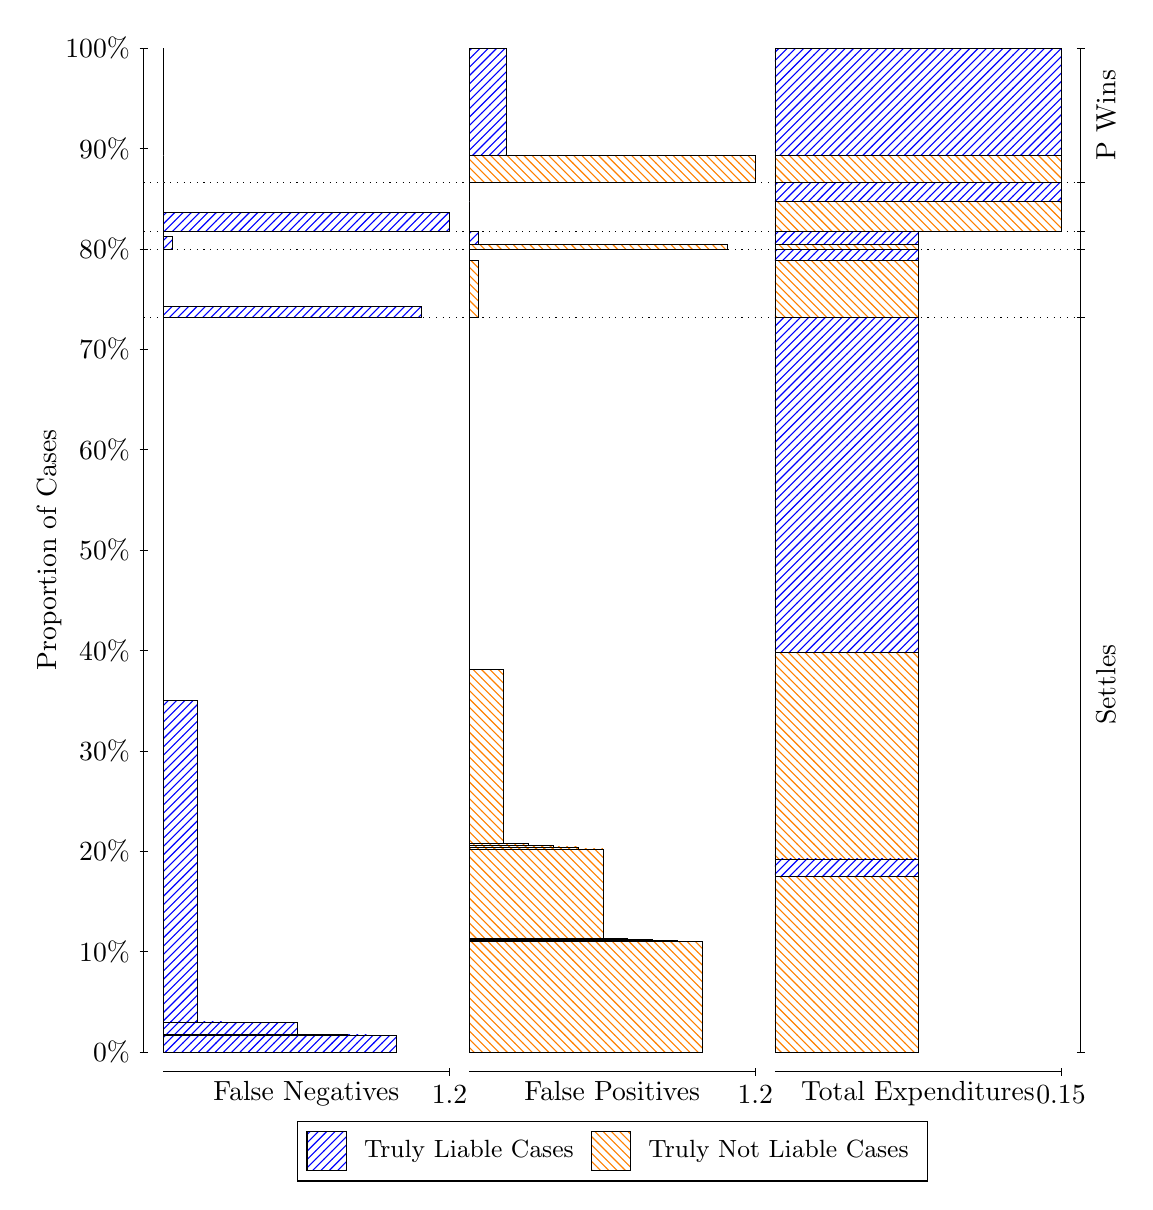
\begin{tikzpicture}
\draw[black, very thin] (1.5,1.75) -- (1.5,14.5);
\node[rotate=90, anchor=center] at (0.3, 8.125) {Proportion of Cases};
\draw[black, very thin] (1.45,1.75) -- (1.55,1.75);
\node[anchor=east] at (1.45, 1.75) {0\%};
\draw[black, very thin] (1.45,3.025) -- (1.55,3.025);
\node[anchor=east] at (1.45, 3.025) {10\%};
\draw[black, very thin] (1.45,4.3) -- (1.55,4.3);
\node[anchor=east] at (1.45, 4.3) {20\%};
\draw[black, very thin] (1.45,5.575) -- (1.55,5.575);
\node[anchor=east] at (1.45, 5.575) {30\%};
\draw[black, very thin] (1.45,6.85) -- (1.55,6.85);
\node[anchor=east] at (1.45, 6.85) {40\%};
\draw[black, very thin] (1.45,8.125) -- (1.55,8.125);
\node[anchor=east] at (1.45, 8.125) {50\%};
\draw[black, very thin] (1.45,9.4) -- (1.55,9.4);
\node[anchor=east] at (1.45, 9.4) {60\%};
\draw[black, very thin] (1.45,10.675) -- (1.55,10.675);
\node[anchor=east] at (1.45, 10.675) {70\%};
\draw[black, very thin] (1.45,11.95) -- (1.55,11.95);
\node[anchor=east] at (1.45, 11.95) {80\%};
\draw[black, very thin] (1.45,13.225) -- (1.55,13.225);
\node[anchor=east] at (1.45, 13.225) {90\%};
\draw[black, very thin] (1.45,14.5) -- (1.55,14.5);
\node[anchor=east] at (1.45, 14.5) {100\%};

\draw[black, very thin] (13.4,1.75) -- (13.4,14.5);
\draw[black, very thin] (13.35,1.75) -- (13.45,1.75);
\node[anchor=west] at (13.35, 1.75) {};
\draw[black, very thin] (13.35,11.078) -- (13.45,11.078);
\node[anchor=west] at (13.35, 11.078) {};
\draw[black, very thin] (13.35,11.942) -- (13.45,11.942);
\node[anchor=west] at (13.35, 11.942) {};
\draw[black, very thin] (13.35,12.174) -- (13.45,12.174);
\node[anchor=west] at (13.35, 12.174) {};
\draw[black, very thin] (13.35,12.791) -- (13.45,12.791);
\node[anchor=west] at (13.35, 12.791) {};
\draw[black, very thin] (13.35,14.5) -- (13.45,14.5);
\node[anchor=west] at (13.35, 14.5) {};

\draw[black, very thin, pattern color=blue, pattern=north east lines] (1.75,1.75) rectangle (4.712,1.9655);
\draw[black, very thin, pattern color=blue, pattern=north east lines] (1.75,1.9655) rectangle (4.396,1.9681);
\draw[black, very thin, pattern color=blue, pattern=north east lines] (1.75,1.9681) rectangle (4.0801,1.9709);
\draw[black, very thin, pattern color=blue, pattern=north east lines] (1.75,1.9709) rectangle (3.7641,1.9739);
\draw[black, very thin, pattern color=blue, pattern=north east lines] (1.75,1.9739) rectangle (3.4482,2.1287);
\draw[black, very thin, pattern color=blue, pattern=north east lines] (1.75,2.1287) rectangle (3.1322,2.1295);
\draw[black, very thin, pattern color=blue, pattern=north east lines] (1.75,2.1295) rectangle (2.8163,2.1302);
\draw[black, very thin, pattern color=blue, pattern=north east lines] (1.75,2.1302) rectangle (2.5004,2.131);
\draw[black, very thin, pattern color=blue, pattern=north east lines] (1.75,2.131) rectangle (2.1844,6.2173);
\draw[black, very thin, pattern color=orange, pattern=north west lines] (1.75,6.2173) rectangle (1.75,11.078);
\draw[black, very thin, pattern color=blue, pattern=north east lines] (1.75,11.078) rectangle (5.0279,11.214);
\draw[black, very thin, pattern color=orange, pattern=north west lines] (1.75,11.214) rectangle (1.75,11.942);
\draw[black, very thin, pattern color=blue, pattern=north east lines] (1.75,11.942) rectangle (1.8685,12.105);
\draw[black, very thin, pattern color=orange, pattern=north west lines] (1.75,12.105) rectangle (1.75,12.174);
\draw[black, very thin, pattern color=blue, pattern=north east lines] (1.75,12.174) rectangle (5.3833,12.417);
\draw[black, very thin, pattern color=orange, pattern=north west lines] (1.75,12.417) rectangle (1.75,12.791);
\draw[black, very thin, pattern color=orange, pattern=north west lines] (1.75,12.791) rectangle (1.75,13.135);
\draw[black, very thin, pattern color=blue, pattern=north east lines] (1.75,13.135) rectangle (1.75,14.5);
\draw[black, very thin, pattern color=orange, pattern=north west lines] (5.6333,1.75) rectangle (8.5953,3.1574);
\draw[black, very thin, pattern color=orange, pattern=north west lines] (5.6333,3.1574) rectangle (8.2793,3.1679);
\draw[black, very thin, pattern color=orange, pattern=north west lines] (5.6333,3.1679) rectangle (7.9634,3.1786);
\draw[black, very thin, pattern color=orange, pattern=north west lines] (5.6333,3.1786) rectangle (7.6475,3.1893);
\draw[black, very thin, pattern color=orange, pattern=north west lines] (5.6333,3.1893) rectangle (7.3315,4.3284);
\draw[black, very thin, pattern color=orange, pattern=north west lines] (5.6333,4.3284) rectangle (7.0156,4.3286);
\draw[black, very thin, pattern color=orange, pattern=north west lines] (5.6333,4.3286) rectangle (7.0156,4.3535);
\draw[black, very thin, pattern color=orange, pattern=north west lines] (5.6333,4.3535) rectangle (6.6996,4.3773);
\draw[black, very thin, pattern color=orange, pattern=north west lines] (5.6333,4.3773) rectangle (6.3837,4.3996);
\draw[black, very thin, pattern color=orange, pattern=north west lines] (5.6333,4.3996) rectangle (6.0678,6.6103);
\draw[black, very thin, pattern color=blue, pattern=north east lines] (5.6333,6.6103) rectangle (5.6333,11.078);
\draw[black, very thin, pattern color=orange, pattern=north west lines] (5.6333,11.078) rectangle (5.7518,11.805);
\draw[black, very thin, pattern color=blue, pattern=north east lines] (5.6333,11.805) rectangle (5.6333,11.942);
\draw[black, very thin, pattern color=orange, pattern=north west lines] (5.6333,11.942) rectangle (8.9112,12.011);
\draw[black, very thin, pattern color=blue, pattern=north east lines] (5.6333,12.011) rectangle (5.7518,12.174);
\draw[black, very thin, pattern color=orange, pattern=north west lines] (5.6333,12.174) rectangle (5.6333,12.548);
\draw[black, very thin, pattern color=blue, pattern=north east lines] (5.6333,12.548) rectangle (5.6333,12.791);
\draw[black, very thin, pattern color=orange, pattern=north west lines] (5.6333,12.791) rectangle (9.2667,13.135);
\draw[black, very thin, pattern color=blue, pattern=north east lines] (5.6333,13.135) rectangle (6.1072,14.5);
\draw[black, very thin, pattern color=orange, pattern=north west lines] (9.5167,1.75) rectangle (11.333,3.983);
\draw[black, very thin, pattern color=blue, pattern=north east lines] (9.5167,3.983) rectangle (11.333,4.2011);
\draw[black, very thin, pattern color=orange, pattern=north west lines] (9.5167,4.2011) rectangle (11.333,6.8284);
\draw[black, very thin, pattern color=blue, pattern=north east lines] (9.5167,6.8284) rectangle (11.333,11.078);
\draw[black, very thin, pattern color=orange, pattern=north west lines] (9.5167,11.078) rectangle (11.333,11.805);
\draw[black, very thin, pattern color=blue, pattern=north east lines] (9.5167,11.805) rectangle (11.333,11.942);
\draw[black, very thin, pattern color=orange, pattern=north west lines] (9.5167,11.942) rectangle (11.333,12.011);
\draw[black, very thin, pattern color=blue, pattern=north east lines] (9.5167,12.011) rectangle (11.333,12.174);
\draw[black, very thin, pattern color=orange, pattern=north west lines] (9.5167,12.174) rectangle (13.15,12.548);
\draw[black, very thin, pattern color=blue, pattern=north east lines] (9.5167,12.548) rectangle (13.15,12.791);
\draw[black, very thin, pattern color=orange, pattern=north west lines] (9.5167,12.791) rectangle (13.15,13.135);
\draw[black, very thin, pattern color=blue, pattern=north east lines] (9.5167,13.135) rectangle (13.15,14.5);
\draw[black, dotted] (1.5,11.078) -- (13.4,11.078);
\draw[black, dotted] (1.5,11.942) -- (13.4,11.942);
\draw[black, dotted] (1.5,12.174) -- (13.4,12.174);
\draw[black, dotted] (1.5,12.791) -- (13.4,12.791);
\draw[black, very thin] (1.75,1.5) -- (5.3833,1.5);
\node[anchor=north] at (3.5667, 1.5) {False Negatives};
\draw[black, very thin] (5.3833,1.45) -- (5.3833,1.55);
\node[anchor=north] at (5.3833, 1.45) {1.2};

\draw[black, very thin] (5.6333,1.5) -- (9.2667,1.5);
\node[anchor=north] at (7.45, 1.5) {False Positives};
\draw[black, very thin] (9.2667,1.45) -- (9.2667,1.55);
\node[anchor=north] at (9.2667, 1.45) {1.2};

\draw[black, very thin] (9.5167,1.5) -- (13.15,1.5);
\node[anchor=north] at (11.333, 1.5) {Total Expenditures};
\draw[black, very thin] (13.15,1.45) -- (13.15,1.55);
\node[anchor=north] at (13.15, 1.45) {0.15};

\node[black, centered, rotate=90] at (13.72, 6.4138) {Settles};



\node[black, centered, rotate=90] at (13.72, 13.646) {P Wins};

\draw (7.449999999999999,1.5) node[draw=none] (baseCoordinate) {};
\begin{scope}[align=center]
        \matrix[scale=0.5, draw=black, below=0.5cm of baseCoordinate, nodes={draw}, column sep=0.1cm]{
            \node[rectangle, draw, minimum width=0.5cm, minimum height=0.5cm, pattern=north east lines, pattern color=blue] {}; &
            \node[draw=none, font=\small] (B) {Truly Liable Cases}; &
            \node[rectangle, draw, minimum width=0.5cm, minimum height=0.5cm, pattern=north west lines, pattern color=orange] {}; &
            \node[draw=none, font=\small] (B) {Truly Not Liable Cases}; \\
            };
\end{scope}

\end{tikzpicture}
\end{document}